\documentclass{article}
\usepackage{xcolor}
\usepackage{tikz}
\usepackage[cache=false]{minted}
\usepackage{listings}
\lstset{
	language=[LaTeX]TeX,breaklines=true,
	basicstyle=\tt\scriptsize,
	keywordstyle=\color{blue},
	identifierstyle=\color{magenta},
	language=[LaTeX]TeX,breaklines=true,
	basicstyle=\tt\footnotesize,
	keywordstyle=\color{blue},
	identifierstyle=\color{red},}
\usepackage{accsupp}
\newcommand*{\noaccsupp}[1]{\BeginAccSupp{ActualText={}}#1\EndAccSupp{}}
\usepackage{showexpl}
\lstset
{
	numbers=left,
	numbersep=1em,
	numberstyle=\footnotesize\color{blue}\noaccsupp,% to hide number lines
	frame=single,
	framesep=\fboxsep,% expands outward, cannot affect if frame=none
	framerule=\fboxrule,% expands outward, cannot affect if frame=none
	rulecolor=\color{red},% cannot affect if frame=none
	xleftmargin=\dimexpr\fboxsep+\fboxrule\relax,
	xrightmargin=\dimexpr\fboxsep+\fboxrule\relax,
	breaklines=true,
	breakindent=0pt,
	tabsize=2,
	columns=flexible,
	language={[LaTeX]TeX},
	basicstyle=\small\ttfamily\hbox{},
	keywordstyle=\color{blue},
	backgroundcolor=\color{blue!15},
	pos=b,
	explpreset={},
}
\parindent=0em
\begin{document}
%	\maketitle
{\LARGE \textbf{\textcolor{blue}{Mewarnai teks di \LaTeXe}}}
\section*{Menggunakan paket minted}
\begin{minted}{latex}
\documentclass{class}	
\begin{document}
\end{document}
\end{minted}
\section*{Menggunakan paket listing }
\begin{lstlisting}
\documentclass{class}	
\begin{document}
\end{document}
\end{lstlisting}
\section*{Menggunakan paket showexpl }
\begin{LTXexample}[width=.5\linewidth,pos=r]
	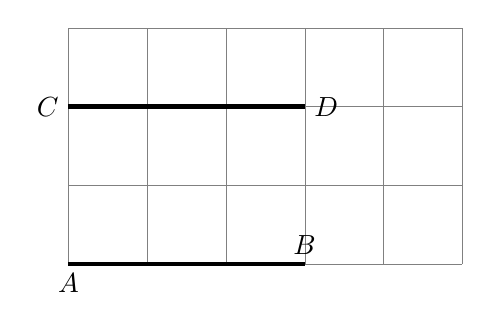
\begin{tikzpicture}
		\draw[ultra thin,gray] (0,0) grid (5,3);
		\coordinate[label=below:$A$] (A) at (0,0);
		\coordinate[label=above:$B$] (B) at (3,0);
		\draw [ultra thick] (A) -- (B);
		\coordinate[label=left:$C$] (C) at (0,2);
		\coordinate[label=right:$D$] (D) at (3,2);
		\draw [ultra thick] (C) -- (D);
	\end{tikzpicture}
\end{LTXexample}
\end{document}